
%(BEGIN_QUESTION)
% Copyright 2006, Tony R. Kuphaldt, released under the Creative Commons Attribution License (v 1.0)
% This means you may do almost anything with this work of mine, so long as you give me proper credit

Her vises et snitt av en enkel trykkrepeater, en enhet som brukes til å kopiere trykket inne i en lukket prosesstank til et rent pneumatisk (luft)trykk, slik at det kan avleses på et fjernmontert manometer:

$$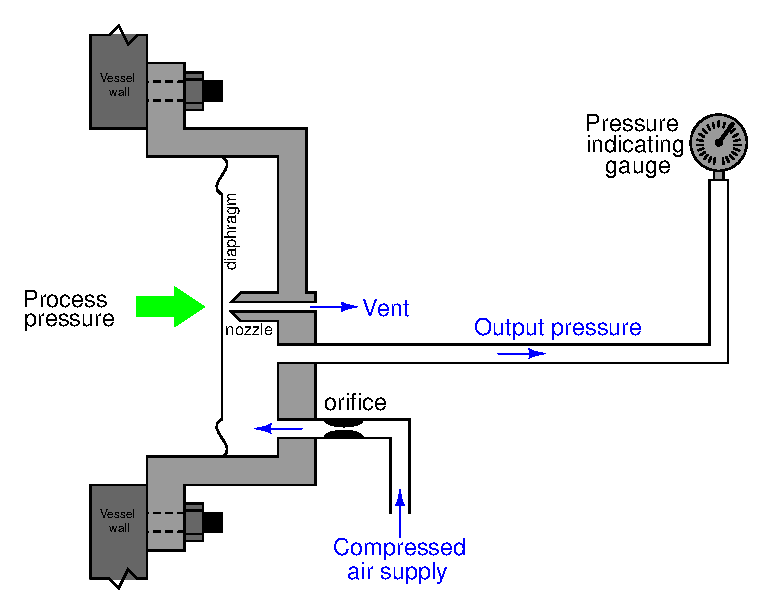
\includegraphics[width=15.5cm]{i00199x01.eps}$$

Beskriv steg for steg hvordan denne enheten responderer på økende prosesstrykk.  Hint: membranen i denne enheten er ``slakk'', det vil si at den har neglisjerbar fjæreffekt.  Dermed er selv små trykkforskjeller nok til å flytte membranen betydelig.

Forklar også hvor en slik enhet er ønskelig å bruke, i stedet for å koble manometeret direkte til prosesstanken.

\underbar{file i00199}
%(END_QUESTION)





%(BEGIN_ANSWER)

Når prosesstrykket øker, øker også kraften som presser membranen mot høyre.  Da beveger membranen seg nærmere dysen, som blir mer strupende for luftstrømmen:

$$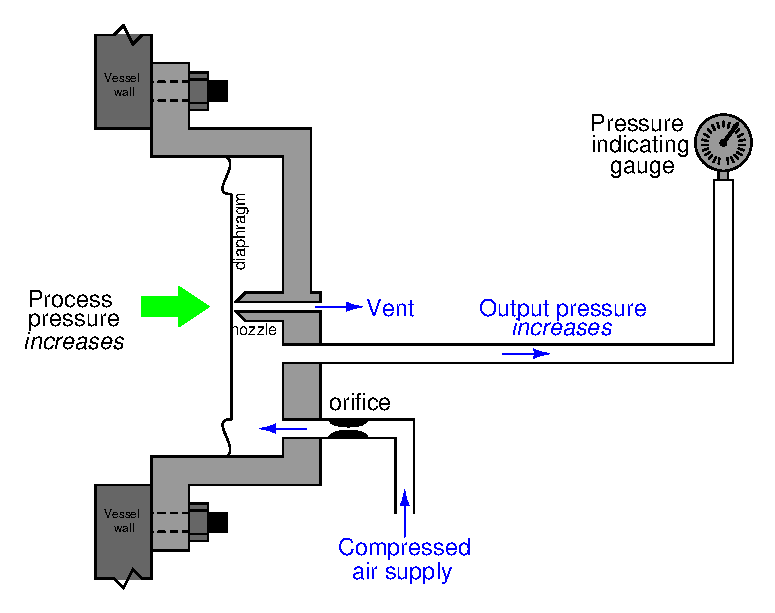
\includegraphics[width=15.5cm]{i00199x02.eps}$$

Når luftstrømmen gjennom dysen reduseres, øker ``baktrykket'' som bygges opp av forsyningsluften gjennom orifice.  Dette økte baktrykket presser membranen mot venstre, mot prosesstrykket, til membranen begynner å trekke seg bort fra dysen og et nytt likevektspunkt nås:

$$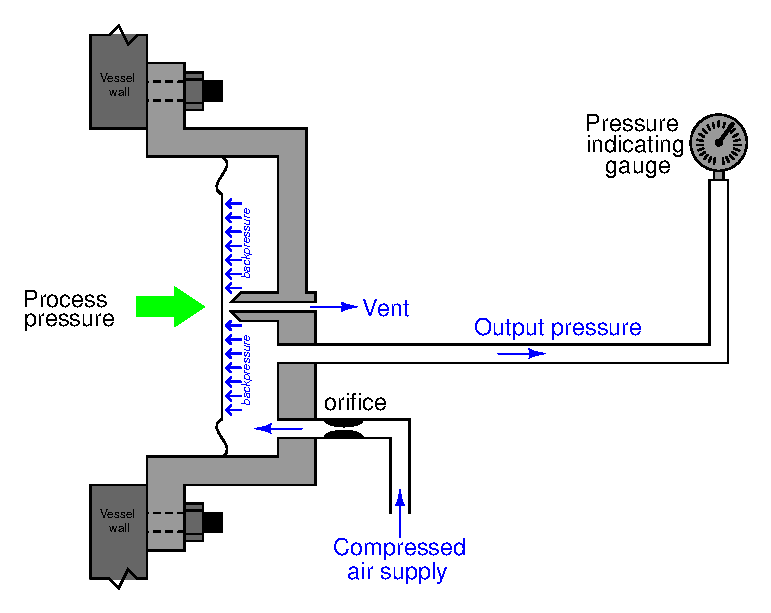
\includegraphics[width=15.5cm]{i00199x03.eps}$$

Siden både prosesstrykket og luftens baktrykk virker på samme membranareal, oppstår kraftbalanse når trykkene er like.  Dermed speiler, eller ``repeterer'', luftutgangen (målt med fjerninstrument) prosesstrykket.

\vskip 10pt

Typiske anvendelser for trykkrepeatere finnes i biofarmasi- og næringsmiddelindustri.  Dersom et manometer kobles direkte til prosesstanken, vil impulsrøret mellom manometer og tank uunngåelig holde igjen noe prosessvæske.  I biofarmasøytiske og næringsmiddelprosesser vil bakterier vokse i stillestående prosessvæske, og slike rørstrekk kan bli reservoar for skadelige bakterier som kontaminerer senere batcher i tanken.

Den flushmonterte membranen i en trykkrepeater er enkel å rengjøre med CIP-prosedyrer (clean-in-place) som brukes på prosesstanker.  På prosessiden finnes ingen spalter eller lommer hvor væske blir stående, og trykkrepeatere eliminerer dermed problemet med bakteriekontaminasjon.

%(END_ANSWER)





%(BEGIN_NOTES)

Den pneumatiske repeateren er et av de enkleste eksemplene på et kraftbalanseinstrument.  Når studenter forstår negativ tilbakekobling i et pneumatisk system, er de forberedt på mer komplekse kraft- og momentbalanserte mekanismer.

Et godt oppfølgingsspørsmål er hvilket forsyningstrykk som kreves for stabil drift.  Dette ligner spørsmålet om hvor høy forsyningsspenning en op-amp må ha når den brukes som spenningsfølger.  I begge tilfeller må forsyningen ligge litt over høyeste signal som skal måles.

\vskip 10pt

For et praktisk eksempel på en pneumatisk trykkrepeater, se Foxboro/Eckhart modell 139PP.

%INDEX% Measurement, pressure: pneumatic repeater

%(END_NOTES)

